\documentclass[11pt]{article}

\usepackage[a4paper,margin=1in]{geometry}
\usepackage{amsmath,amssymb,amsthm,mathtools}
\usepackage{bm}
\usepackage{booktabs}
\usepackage{graphicx}
\usepackage{hyperref}
\usepackage[numbers]{natbib}
\usepackage{tikz-cd}

\newcommand{\ones}{\mathbf{1}}
\newcommand{\diag}{\operatorname{diag}}
\newcommand{\KL}{\operatorname{KL}}
\newcommand{\Tset}{\mathcal{T}}
\newcommand{\Piset}{\Pi}
\newtheorem{proposition}{Proposition}

\title{Tutorial on Discrete Diffusion\\[0.3em]\large Forward Noising, Backward Couplings, Learning, and Operator Matching}
\author{}
\date{}

\begin{document}
\maketitle

\section{Forward Noising Process}
We work on a finite state space $\mathcal{X}=\{1,\dots,n\}$. Let
\[
h^t\in\mathbb{R}_+^n,\qquad \sum_{i=1}^n h_i^t=1
\]
be the histogram (marginal law) at time $t$.

The forward kernel is row-stochastic:
\[
P\in\mathbb{R}_+^{n\times n},\qquad P_{ij}=\mathbb{P}(X_{t+1}=j\mid X_t=i),\qquad P\ones=\ones.
\]
Forward marginals follow
\begin{equation}
\label{eq:forward-recursion}
h^{t+1}=P^\top h^t,
\end{equation}
for $t=0,\dots,T-1$, hence we have $T+1$ histograms $(h^0,\dots,h^T)$.

\paragraph{Examples of forward kernels (detailed).}
\begin{itemize}
\item \textbf{Local geometric kernel.}
For interior states, mass is split on neighbors and self:
\[
P_{ij}=\frac13\,\mathbf{1}_{j\in\{i-1,i,i+1\}},
\]
with boundary rows set by a chosen convention (reflecting or periodic).
This kernel encodes local motion and typically smooths histograms spatially.

\item \textbf{Gaussian convolution kernel.}
For a bandwidth $\sigma>0$,
\[
P_{ij}\propto \exp\!\left(-\frac{(i-j)^2}{2\sigma^2}\right),
\qquad
\sum_j P_{ij}=1.
\]
Large $\sigma$ gives stronger global mixing; small $\sigma$ remains local.

\item \textbf{Masking/absorbing kernel.}
Choose a special absorbing state $n$ and set
\[
P_{ii}=1-\varepsilon,\quad P_{in}=\varepsilon\ (i\neq n),\quad P_{nn}=1.
\]
The process progressively transfers mass toward state $n$.
\end{itemize}

\paragraph{Forward particle process.}
Define one Markov process $(X^t)_{t=0}^T$ by
\[
X^0\sim h^0,
\qquad
X^{t+1}\sim P\big(X^t,\cdot\big).
\]
Then
\[
h^t=\mathrm{Law}(X^t),
\]
and \eqref{eq:forward-recursion} is exactly the evolution of this law.

\paragraph{Forward figures.}
The script \texttt{figures/figures.py} generates forward visualizations using the same Gaussian forward kernel as the notebook,
\[
P_{ij}\propto \exp\!\left(-\frac{(i-j)^2}{2\sigma^2}\right),\qquad \sigma=0.75.
\]
\begin{figure}[h]
\centering
\begin{minipage}{0.48\linewidth}
\centering
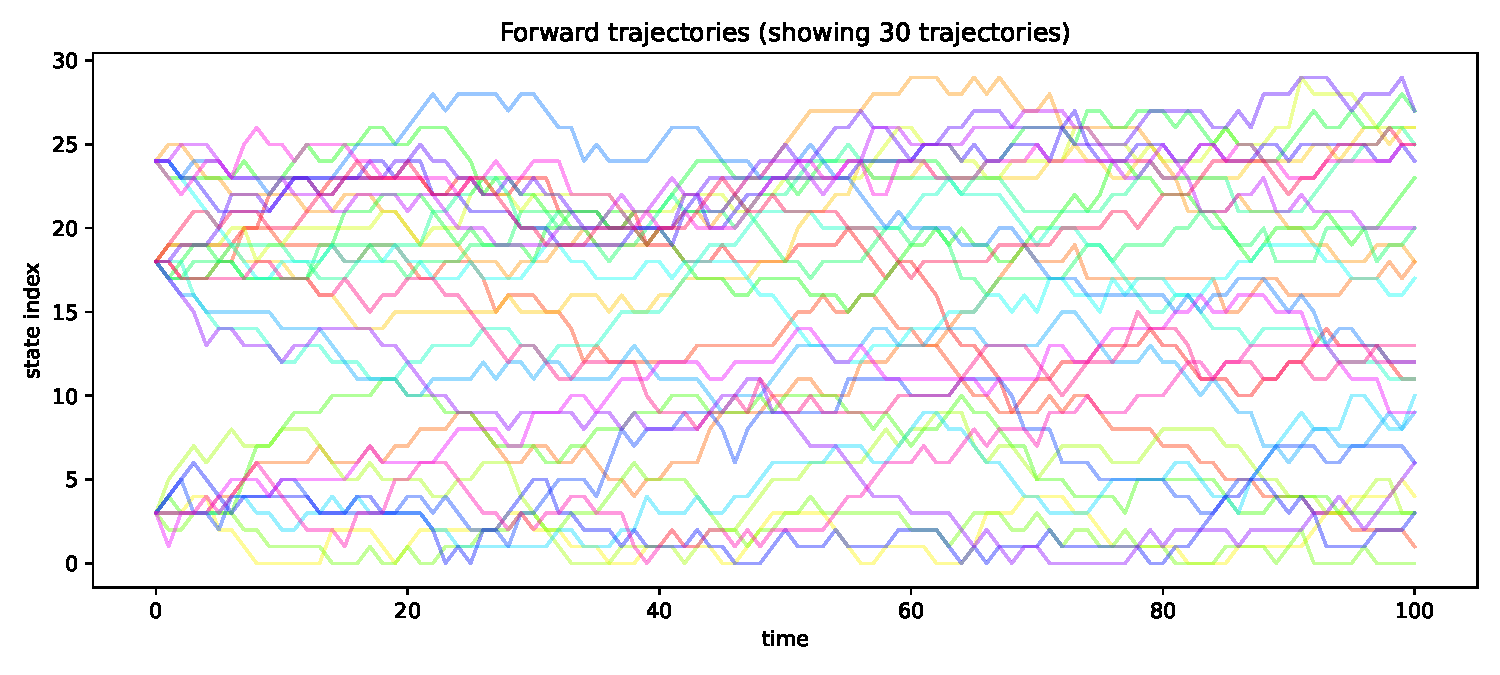
\includegraphics[width=\linewidth]{figures/forward_trajectories.pdf}
\end{minipage}\hfill
\begin{minipage}{0.48\linewidth}
\centering
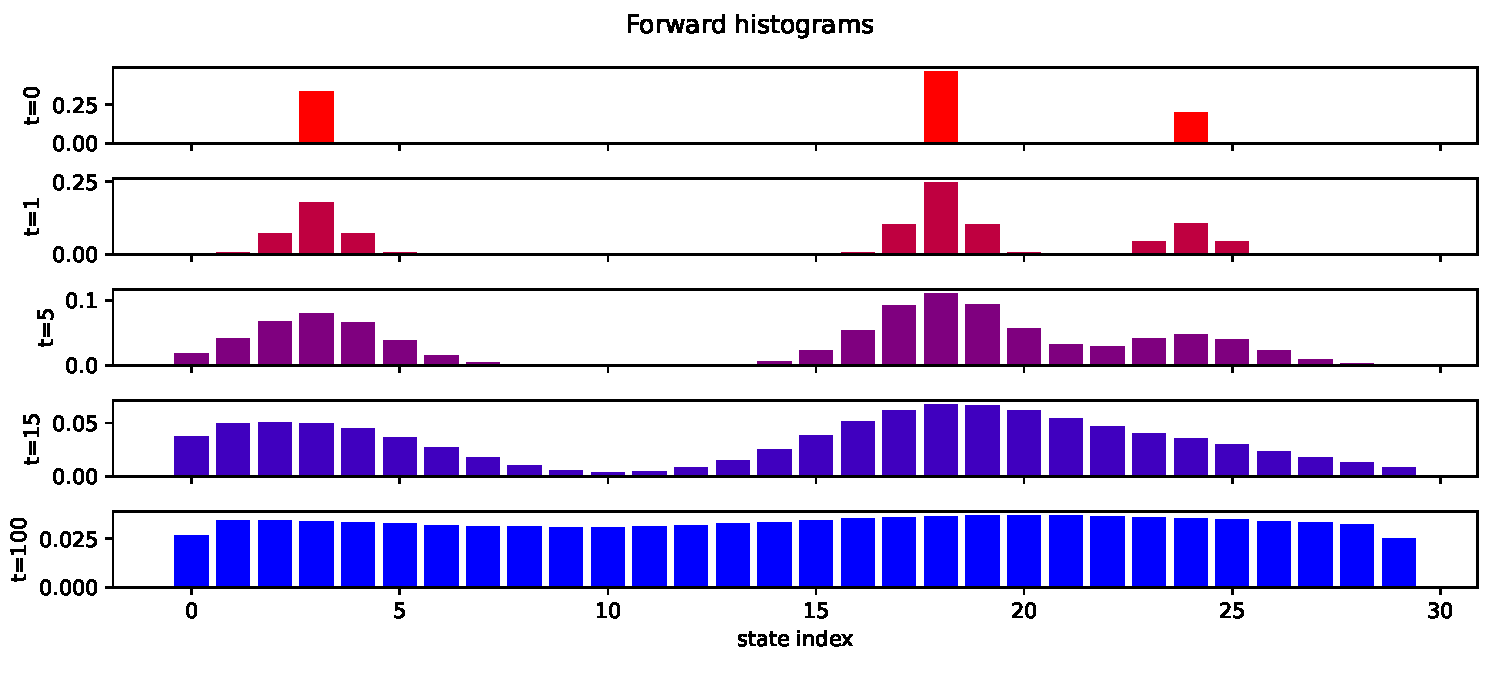
\includegraphics[width=\linewidth]{figures/forward_histograms.pdf}
\end{minipage}
\caption{Forward process (left: trajectories, right: vertically stacked histogram snapshots) generated with the Gaussian kernel $P$.}
\label{fig:forward-figures}
\end{figure}

\section{Backward Kernels and Coupling}
\subsection{Admissible kernels between consecutive marginals}
Fix $a,b\in\Delta_n$ (probability simplex). Define
\[
\Tset(a,b)=\left\{K\in\mathbb{R}_+^{n\times n}:\ K\ones=\ones,\ K^\top a=b\right\}.
\]
Thus $P\in\Tset(h^t,h^{t+1})$ by \eqref{eq:forward-recursion}.

An inverse (backward) kernel at step $t$ is any
\[
Q^t\in\Tset(h^{t+1},h^t),
\]
that is,
\[
Q^t\ones=\ones,
\qquad
(Q^t)^\top h^{t+1}=h^t.
\]
So there are exactly $T$ backward kernels $Q^0,\dots,Q^{T-1}$ connecting $t+1\to t$.

\subsection{Backward particle process}
Given admissible kernels $(Q^t)_{t=0}^{T-1}$, define $(Y^t)_{t=0}^T$ backward by
\[
Y^T\sim h^T,\qquad
Y^t\sim Q^t(Y^{t+1},\cdot),\quad t=T-1,\dots,0.
\]
If each $Q^t\in\Tset(h^{t+1},h^t)$, then
\[
\mathrm{Law}(Y^t)=h^t,\qquad t=0,\dots,T,
\]
so backward recursion terminates at $h^0$.

\subsection{Bayes inverse as a canonical admissible reverse kernel}
\paragraph{Definition (Bayes kernel).}
Given a forward chain with kernel $P$ and marginals $(h^t)$, the Bayes kernel at time $t$ is
\[
Q^{\mathrm B,t}_{ij}\coloneqq
\mathbb{P}(X^t=j\mid X^{t+1}=i).
\]

\begin{proposition}
Let $a=h^t$, $b=h^{t+1}$ and $P\in\Tset(a,b)$. Then for $b_i>0$,
\begin{equation}
\label{eq:bayes-entry}
Q^{\mathrm B}_{ij}=\frac{a_jP_{ji}}{b_i}.
\end{equation}
In matrix form,
\begin{equation}
\label{eq:bayes-diag}
Q^{\mathrm B}=\diag(b)^+P^\top\diag(a).
\end{equation}
Moreover, $Q^{\mathrm B}\in\Tset(b,a)$, i.e. it is an admissible inverse kernel.
\end{proposition}

\paragraph{Bayesian inversion map.}
Define
\[
\mathcal B_{a,b}:\Tset(a,b)\to\Tset(b,a),\qquad
\mathcal B_{a,b}(K)\coloneqq \diag(b)^+K^\top\diag(a).
\]
On supports where $a_i,b_i>0$, this map is a bijection, with inverse
\[
\mathcal B_{a,b}^{-1}(L)=\mathcal B_{b,a}(L)=\diag(a)^+L^\top\diag(b).
\]
Therefore Bayesian inversion is not only a way to build one reverse kernel from $P$; it defines a one-to-one correspondence between admissible forward kernels and admissible backward kernels.

When $b_i=0$, row $i$ does not affect $(Q^{\mathrm B})^\top b$ and can be set by pseudo-inverse convention plus row renormalization.

\paragraph{Backward figures.}
Using $Q^t=\mathcal B_{h^t,h^{t+1}}(P)$ at each step, the backward process
\[
Y^T\sim h^T,\qquad Y^t\sim Q^t(Y^{t+1},\cdot)
\]
has marginals $h^t$ for $t=T,\dots,0$. Figure~\ref{fig:backward-figures} displays backward trajectories (left) and empirical histograms of $Y^t$ (right), generated with the Bayes inverse kernels associated with the same Gaussian forward kernel $P$.
\begin{figure}[h]
\centering
\begin{minipage}{0.48\linewidth}
\centering
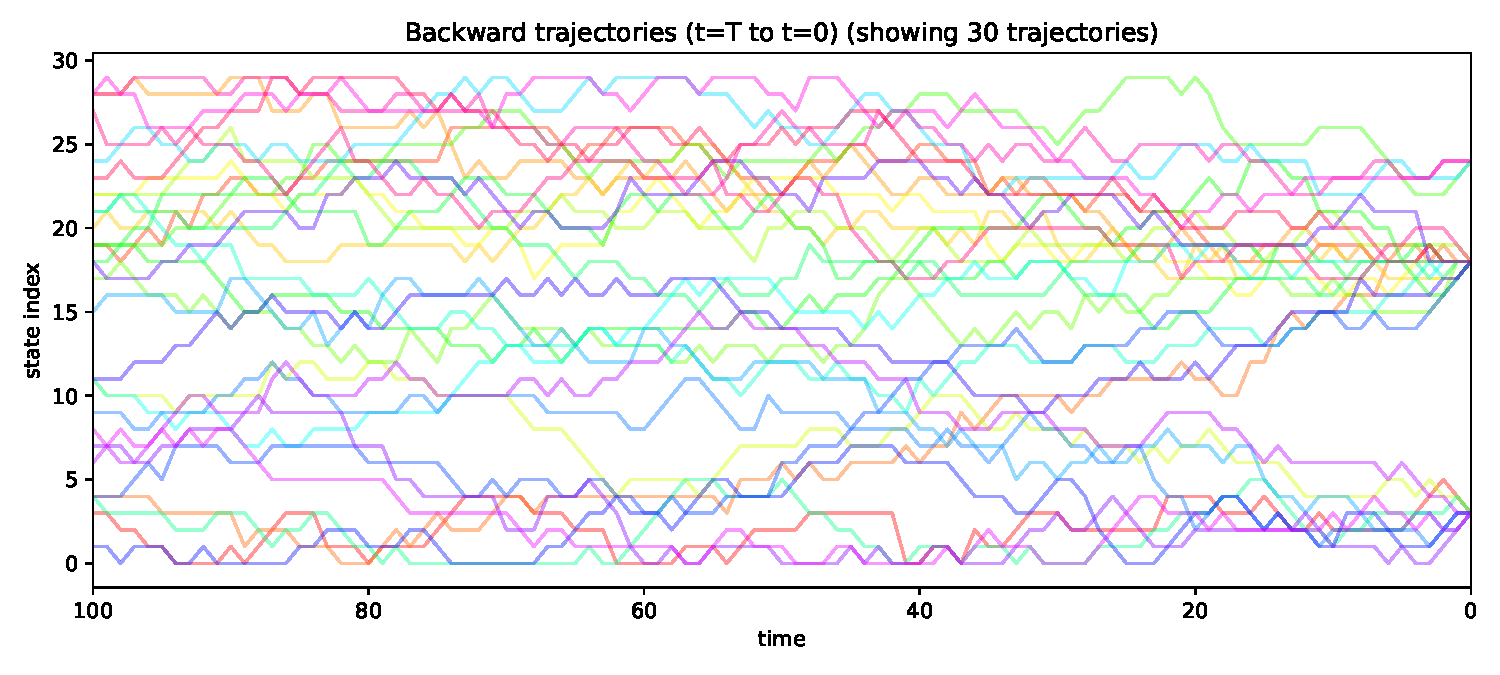
\includegraphics[width=\linewidth]{figures/backward_trajectories.pdf}
\end{minipage}\hfill
\begin{minipage}{0.48\linewidth}
\centering
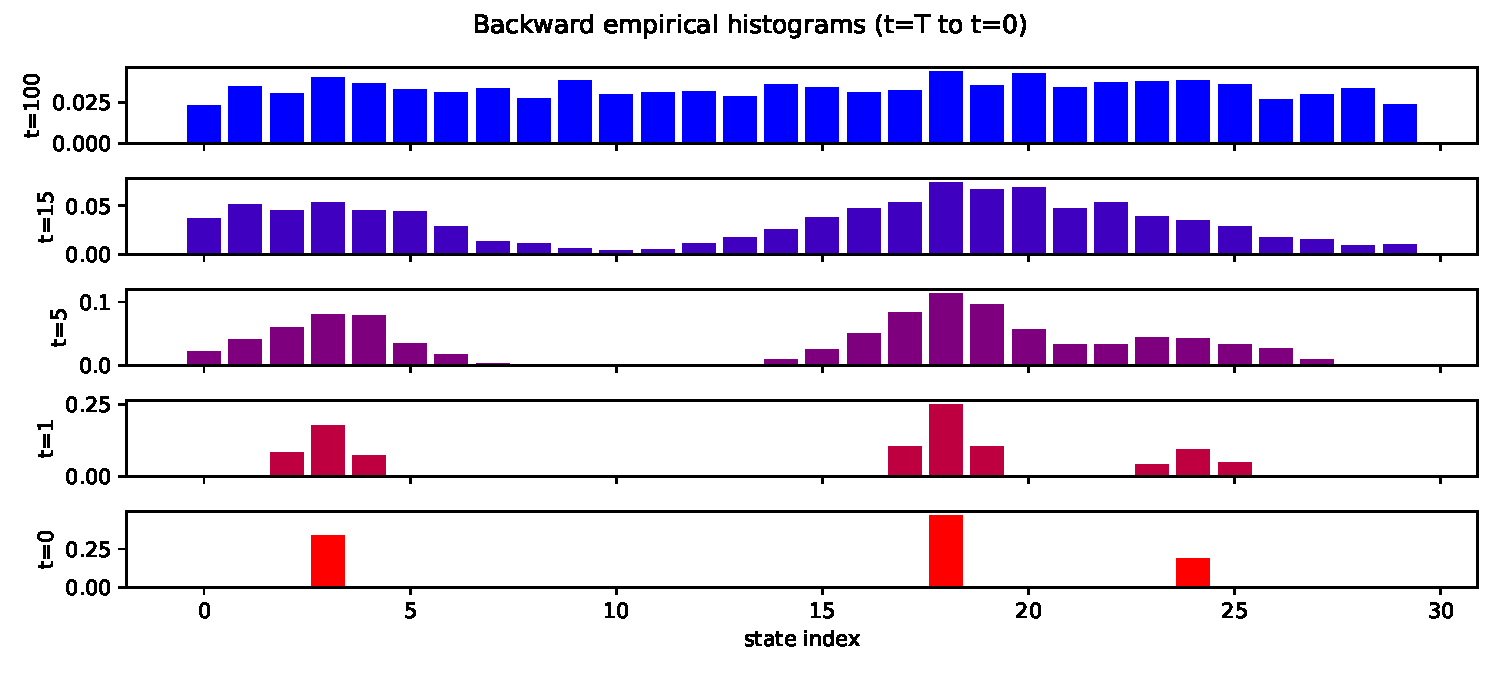
\includegraphics[width=\linewidth]{figures/backward_histograms.pdf}
\end{minipage}
\caption{Backward process (left: trajectories in backward time, right: vertically stacked empirical histogram snapshots of $Y_t$). Kernel: Bayes inverse of the Gaussian forward kernel $P$.}
\label{fig:backward-figures}
\end{figure}

\subsection{Coupling polytope and bijection with kernels}
Define
\[
\Piset(a,b)=\left\{\pi\in\mathbb{R}_+^{n\times n}:\ \pi\ones=a,\ \pi^\top\ones=b\right\}.
\]

Kernel--coupling bijection (on $\mathrm{supp}(a)$):
\[
\Phi_a:\Tset(a,b)\to\Piset(a,b),\qquad \Phi_a(K)=\diag(a)K,
\]
with inverse
\[
\Phi_a^{-1}(\pi)=\diag(a)^+\pi,
\]
where $\diag(a)^+$ is the diagonal pseudo-inverse ($1/a_i$ if $a_i>0$, else $0$).

Hence choosing a Markov kernel in $\Tset(a,b)$ is equivalent to choosing a coupling in $\Piset(a,b)$.
\paragraph{Interleaving with transposition and Bayes kernel as transposed coupling.}
Let
\[
\mathsf T:\Piset(a,b)\to\Piset(b,a),\qquad \mathsf T(\pi)=\pi^\top.
\]
Define similarly
\[
\Phi_b:\Tset(b,a)\to\Piset(b,a),\qquad \Phi_b(L)=\diag(b)L.
\]
Then the maps commute:
\[
\mathsf T\circ \Phi_a=\Phi_b\circ \mathcal B_{a,b},
\]
equivalently
\[
\mathcal B_{a,b}=\Phi_b^{-1}\circ \mathsf T\circ \Phi_a.
\]
So Bayesian inversion in kernel coordinates is exactly transposition in coupling coordinates. In particular, for $P\in\Tset(a,b)$ with $\pi=\Phi_a(P)=\diag(a)P$, the Bayes kernel is
\[
Q^{\mathrm B}=\Phi_b^{-1}\!\big(\mathsf T(\pi)\big)=\diag(b)^+\pi^\top.
\]
This is summarized by the commutative diagram (with arrows in both directions):
\[
\begin{tikzcd}[column sep=huge,row sep=large]
\Tset(a,b)
  \arrow[r,shift left=0.8ex,"\Phi_a"]
  \arrow[d,shift left=0.8ex,"\mathcal B_{a,b}"]
&
\Piset(a,b)
  \arrow[l,shift left=0.8ex,"\Phi_a^{-1}"]
  \arrow[d,leftrightarrow,"\mathsf T"]
\\
\Tset(b,a)
  \arrow[r,shift left=0.8ex,"\Phi_b"']
  \arrow[u,shift left=0.8ex,"\mathcal B_{b,a}"']
&
\Piset(b,a)
  \arrow[l,shift left=0.8ex,"\Phi_b^{-1}"']
\end{tikzcd}
\]

\section{Learning the Reverse Kernel}
\subsection{Statistical formulation}
Let $Q_\theta^t(i,j)$ be a neural network parameterization such that, for each $(t,i)$,
\[
Q_\theta^t(i,\cdot)\in\Delta_n
\]
(typically enforced by a softmax over $j$).

Assume we observe i.i.d.\ samples
\[
\big(X_k^{t_k},X_k^{t_k+1},t_k\big)_{k=1}^N,
\]
where $t_k$ are i.i.d.\ in $\{0,\dots,T-1\}$ (e.g.\ uniform), and
\[
X_k^{t_k+1}\sim P\!\left(X_k^{t_k},\cdot\right),\qquad
X_k^{t_k}\sim h^{t_k}.
\]
Equivalently, each triplet is drawn from the joint law induced by the forward noising process:
\[
t\sim \pi\ \text{on}\ \{0,\dots,T-1\},\quad
X^t\sim h^t,\quad
X^{t+1}\mid X^t\sim P(X^t,\cdot),
\]
then set $(t_k,X_k^{t_k},X_k^{t_k+1})$ as i.i.d.\ copies of $(t,X^t,X^{t+1})$.
The empirical negative log-likelihood is
\begin{equation}
\label{eq:empirical-loss-user}
L_N(\theta)
\coloneqq
\frac1N\sum_{k=1}^N
\Big[-\log Q_\theta^{t_k}\!\big(X_k^{t_k+1},X_k^{t_k}\big)\Big].
\end{equation}
Let $\theta_N$ be a global minimizer of $L_N$.

\subsection{Population target and consistency interpretation}
Define the Bayes reverse kernels
\[
Q_\star^t(i,j)\coloneqq \mathbb P(X^t=j\mid X^{t+1}=i,\,t),
\]
which coincide with the canonical Bayes inverse from Section 2.
The population risk is
\[
L(\theta)=\mathbb E_{\substack{t\sim\pi\\X^t\sim h^t\\X^{t+1}\mid X^t\sim P(X^t,\cdot)}}\!\left[-\log Q_\theta^{t}(X^{t+1},X^t)\right].
\]

\begin{proposition}[Population NLL decomposition]
Let $Q_\theta^t(i,\cdot)\in\Delta_n$ for all $(t,i)$. Then
\begin{equation}
\label{eq:pop-kl-decomp}
L(\theta)=C+\sum_{t=0}^{T-1}\pi(t)\sum_{i=1}^n h_i^{t+1}\,
\KL\!\big(Q_\star^t(i,\cdot)\,\|\,Q_\theta^t(i,\cdot)\big),
\end{equation}
where
\[
C=\sum_{t=0}^{T-1}\pi(t)\sum_{i=1}^n h_i^{t+1}\,H\!\big(Q_\star^t(i,\cdot)\big)
\]
is independent of $\theta$.
\end{proposition}
\begin{proof}
Condition on $(t,X^{t+1}=i)$ and use $X^t\mid (t,X^{t+1}=i)\sim Q_\star^t(i,\cdot)$:
\[
L(\theta)=\sum_t \pi(t)\sum_i h_i^{t+1}\sum_j
Q_\star^t(i,j)\big[-\log Q_\theta^t(i,j)\big].
\]
Add and subtract $\log Q_\star^t(i,j)$ inside the sum:
\[
\sum_j Q_\star^t(i,j)\big[-\log Q_\theta^t(i,j)\big]
=H(Q_\star^t(i,\cdot))
+\KL(Q_\star^t(i,\cdot)\|Q_\theta^t(i,\cdot)).
\]
Summing over $(t,i)$ gives \eqref{eq:pop-kl-decomp}.
\end{proof}

Therefore, minimizing $L(\theta)$ is equivalent to minimizing
\[
\sum_{t=0}^{T-1}\pi(t)\sum_{i=1}^n h_i^{t+1}\,
\KL\!\big(Q_\star^t(i,\cdot)\,\|\,Q_\theta^t(i,\cdot)\big).
\]

\begin{proposition}[Consistency, informal]
Assume:
\begin{itemize}
\item the model class is rich enough to represent $Q_\star$ (well-specified/universal approximation),
\item empirical risk minimization is statistically consistent (uniform LLN / Glivenko--Cantelli type conditions),
\item optimization finds a global minimizer (or asymptotically equivalent minimizers).
\end{itemize}
Then any limit point of $Q_{\theta_N}$ minimizes $L$ and agrees with $Q_\star^t(i,\cdot)$ for all $(t,i)$ such that $\pi(t)\,h_i^{t+1}>0$.
Hence the limit kernel is admissible:
\[
Q_{\theta^\star}^t\in\Tset(h^{t+1},h^t),\qquad t=0,\dots,T-1.
\]
\end{proposition}

\paragraph{Important practical caveat.}
For finite $N$, minimizing \eqref{eq:empirical-loss-user} enforces row-stochasticity (via softmax) but does \emph{not} guarantee exact marginal constraints
\[
(Q_\theta^t)^\top h^{t+1}=h^t.
\]
Exact admissibility is an asymptotic/population property under the assumptions above, or can be encouraged by explicit constraints/penalties.

\subsection{Neural parameterization example}
For 1D geometric histograms, a simple input encoding is
\[
\mathrm{position}(i)\ \Vert\ (t/T),
\]
with $\mathrm{position}(i)=i/(n-1)$ (or $i/n$). If no spatial prior is available, one may use $\mathrm{position}(i)=\mathrm{onehot}(i)$.
A practical architecture is a 2-layer MLP with one ReLU and a final softmax over $j$
\citep{austin2021structured,campbell2022continuous,bach2025binary,pauline2025foundations}.


\section{Connection with Classical Gaussian Diffusion}
\subsection{Additive Gaussian forward noising}
In continuous state space ($x\in\mathbb R^d$), a standard forward step is
\[
X^{t+\tau}=X^t+\sqrt{2\tau}\,\xi,\qquad \xi\sim\mathcal N(0,I_d),
\]
so
\[
p_\tau(x^{t+\tau}\mid x^t)=\mathcal N(x^t,\,2\tau I_d).
\]
More generally, for an SDE
\[
dX^t=f(X^t,t)\,dt+g(t)\,dW_t,
\]
the short-time kernel is Gaussian with mean $x+\tau f(x,t)$ and covariance $\tau g(t)^2 I_d$.

\subsection{Bayes reverse conditional and score expansion}
Let $p_t$ be the density of $X^t$. By Bayes rule,
\[
p(x^t\mid x^{t+\tau})
\propto
p_\tau(x^{t+\tau}\mid x^t)\,p_t(x^t).
\]
For small $\tau$, a first-order expansion yields a Gaussian approximation
\[
X^t\mid X^{t+\tau}=y
\approx
\mathcal N\!\Big(y-\tau f(y,t)+\tau g(t)^2\nabla_y\log p_t(y),\ \tau g(t)^2 I_d\Big),
\]
where the score is $s_t(y)=\nabla_y\log p_t(y)$.

\subsection{Limit $\tau\to 0$: reverse-time SDE}
Thus sampling from the reverse conditionals converges to the reverse-time SDE
\[
dX^t=\big(f(X^t,t)-g(t)^2\nabla\log p_t(X^t)\big)\,dt+g(t)\,d\bar W_t
\]
(time run backward).
For pure additive Gaussian noising ($f=0$, $g=\sqrt2$):
\[
dX^t=-2\,\nabla\log p_t(X^t)\,dt+\sqrt2\,d\bar W_t,
\]
which is the classical score-based reverse diffusion dynamics.

\section{Fine-Grid and Small-Step Limit: Denoising Form}
We isolate here the 1D fine-grid limit and write the reverse-kernel parameterization directly in terms of a score-like field.

Let
\[
x_i=i\Delta x,\qquad i=1,\dots,n,\qquad \Delta x\to 0\ (n\to\infty),
\]
and consider the simple Gaussian forward step (no drift parameter):
\[
P_{ij}\propto \exp\!\left(-\frac{(x_j-x_i)^2}{4\tau}\right),
\qquad \Delta t=\tau.
\]
In continuous notation this corresponds to
\[
X^{t+\tau}\mid X^t=x \sim \mathcal N(x,2\tau).
\]

Denote by $x'$ the state at time $t+\tau$ and by $x$ the state at time $t$. The Bayes reverse conditional is
\[
q_\star^\tau(x\mid x',t)\propto
\exp\!\left(-\frac{(x'-x)^2}{4\tau}\right)\,p_t(x).
\]
Write $s_t(x')\coloneqq \partial_x\log p_t(x')$. A first-order Taylor expansion
\[
\log p_t(x)=\log p_t(x')+(x-x')\,s_t(x')+O((x-x')^2)
\]
in the $\tau\to0$ regime ($x-x'=O(\sqrt{\tau})$) gives, after completing the square,
\[
q_\star^\tau(x\mid x',t)\approx
\mathcal N\!\big(x'+2\tau s_t(x'),\,2\tau\big).
\]
This gives the rationale for a reverse-kernel model driven by a field $s_\theta^t$:
\begin{equation}
\label{eq:qtheta-discrete-grid}
Q_\theta^t(x_j\mid x_i')
\coloneqq
\frac{\exp\!\left(-\frac{(x_j-x_i'-2\tau s_\theta^t(x_i'))^2}{4\tau}\right)}
{\sum_{\ell=1}^n \exp\!\left(-\frac{(x_\ell-x_i'-2\tau s_\theta^t(x_i'))^2}{4\tau}\right)}.
\end{equation}
So the discrete Bayes inverse kernel is expected to be locally approximated by this shifted-Gaussian family.

\begin{proposition}[One-step NLL in denoising form, formal expansion]
Assume the local approximation above and parameterization \eqref{eq:qtheta-discrete-grid}. Then, up to $o(1)$ terms and additive constants independent of $\theta$,
\[
L_\tau(\theta)
=
\mathbb E\!\big[-\log Q_\theta^t(X^t\mid X^{t+\tau})\big]
=
C_\tau+\frac{1}{4\tau}\,
\mathbb E\!\left[\big(X^t-X^{t+\tau}-2\tau s_\theta^t(X^{t+\tau})\big)^2\right].
\]
Equivalently, defining the denoising target
\[
D_\tau\coloneqq \frac{X^t-X^{t+\tau}}{2\tau},
\]
minimizing $L_\tau$ is equivalent (up to scaling/constants) to minimizing
\[
\mathbb E\!\left[\big(D_\tau-s_\theta^t(X^{t+\tau})\big)^2\right].
\]
\end{proposition}
\begin{proof}[Proof sketch]
Insert \eqref{eq:qtheta-discrete-grid} into $-\log Q_\theta^t(X^t\mid X^{t+\tau})$. The log-normalizer contributes only through terms independent of $X^t$ at leading order, absorbed in $C_\tau$. Expanding the quadratic term yields exactly the stated squared-error form.
\end{proof}

\paragraph{Important clarification on the $\tau\to0$ limit.}
A naive pointwise limit of
\[
\mathbb E\!\left[\big(D_\tau-s_\theta^t(X^{t+\tau})\big)^2\right]
\]
is not finite, because $D_\tau=(X^t-X^{t+\tau})/(2\tau)$ has variance of order $1/\tau$.
Indeed, under $X^{t+\tau}=X^t+\sqrt{2\tau}\,\xi$,
\[
D_\tau=-\frac{\xi}{\sqrt{2\tau}}+O(1),
\]
so the unscaled loss diverges as $\tau\downarrow0$.

The meaningful object is the \emph{excess} risk (or equivalently the $\theta$-dependent part), after removing the diverging noise floor:
\[
L_\tau(\theta)-L_\tau(\theta_\star)
\;\sim\;
\tau\,\mathbb E\!\left[\big(s_\theta^t(X^{t+\tau})-s_t(X^{t+\tau})\big)^2\right].
\]
Hence one does not identify score matching from a single unscaled step; it appears after the proper small-step rescaling and, over a finite horizon, after summing/integrating many steps ($T\sim 1/\tau$):
\[
\sum_{k=0}^{T-1}\!\big(L_\tau^{(k)}(\theta)-L_\tau^{(k)}(\theta_\star)\big)
\;\longrightarrow\;
\int_0^{\mathsf T} w(t)\,
\mathbb E\!\left[\big(s_\theta^t(X^t)-s^t(X^t)\big)^2\right]dt
\]
for an explicit weight $w(t)$ (equal to $1$ in this normalized additive-noise setting).
So your intuition is correct: the score-matching structure is fundamentally a multi-step/time-integrated limit, not a raw one-step $\tau\to0$ limit of $D_\tau$.


\section{Continuous-Time Finite-Chain Formulation and Operator Matching}
\subsection{Continuous-time extension of the finite-state tutorial}
Let $\mathcal X=\{1,\dots,n\}$ and let $(A_t)_{t\in[0,T]}$ be a time-dependent forward generator:
\[
(A_t)_{ij}\ge 0\ (j\neq i),\qquad
(A_t)_{ii}=-\sum_{j\neq i}(A_t)_{ij}.
\]
The forward marginal evolves by the Kolmogorov equation
\[
\frac{d}{dt}h^t=A_t^\top h^t,\qquad h^0\in\Delta_n.
\]
For small step $\tau$, the discrete kernel is
\[
P^t=I+\tau A_t+o(\tau),
\]
which recovers the tutorial recursion $h^{t+\tau}=(P^t)^\top h^t$.

\subsection{Backward generator by infinitesimal Bayes inversion}
Define reverse rates for $i\neq j$ by
\[
(\widetilde A_t)_{ij}
=\frac{h_j^t}{h_i^t}(A_t)_{ji},
\qquad
(\widetilde A_t)_{ii}=-\sum_{j\neq i}(\widetilde A_t)_{ij}.
\]
Then $Q^t=I+\tau \widetilde A_t+o(\tau)$ is the infinitesimal analogue of Bayes reverse kernels.
Moreover, $(h^t)$ is invariant for reverse-time dynamics in the sense
\[
\frac{d}{dt}h^t=-\widetilde A_t^\top h^t.
\]
This is the continuous-time counterpart of $Q^t\in\Tset(h^{t+\tau},h^t)$.

\subsection{Operator matching viewpoint in finite Markov chains}
For test functions $\varphi:\mathcal X\to\mathbb R$, define forward/backward operators
\[
(\mathcal L_t\varphi)(i)=\sum_j (A_t)_{ij}\big(\varphi(j)-\varphi(i)\big),
\]
\[
(\widetilde{\mathcal L}_t\varphi)(i)=\sum_j (\widetilde A_t)_{ij}\big(\varphi(j)-\varphi(i)\big).
\]
The weak-form evolution is
\[
\frac{d}{dt}\langle h^t,\varphi\rangle=\langle h^t,\mathcal L_t\varphi\rangle,
\]
which is the finite-state analogue of the weak continuity-equation formulation used in operator flow matching.

To make operator matching identifiable, one must average over a rich family of test functions.
Let $\Phi\subset \mathbb R^{\mathcal X}$ be a function class and let $\rho$ be a sampling law on $\Phi$.
Given a parametric reverse generator $\widetilde A_\theta(t)$ (equivalently operator $\widetilde{\mathcal L}_\theta$), define
\[
\mathcal J_{\mathrm{op}}(\theta)
\coloneqq
\mathbb E_{t}\,\mathbb E_{\varphi\sim\rho}\,\mathbb E_{i\sim h^t}\Big[
\big((\widetilde{\mathcal L}_\theta)_t\varphi(i)-(\widetilde{\mathcal L}_\star)_t\varphi(i)\big)^2
\Big],
\]
where $\widetilde{\mathcal L}_\star$ is the Bayes reverse operator.
In practice, $\rho$ can be:
\begin{itemize}
\item uniform over a finite basis $\Phi=\{\varphi_m\}_{m=1}^M$ (e.g., canonical basis or low-frequency graph modes), or
\item a random-feature distribution on functions.
\end{itemize}
Then
\[
\mathcal J_{\mathrm{op}}(\theta)\approx \frac1M\sum_{m=1}^M
\mathbb E_t\mathbb E_{i\sim h^t}\!\left[
\big((\widetilde{\mathcal L}_\theta)_t\varphi_m(i)-(\widetilde{\mathcal L}_\star)_t\varphi_m(i)\big)^2
\right].
\]
This is the finite-chain specialization of matching transport operators/vector fields rather than directly matching full conditional distributions.

\paragraph{Link with kernel log-likelihood training.}
For small $\tau$, minimizing transition NLL for kernels
\[
Q_\theta^t=I+\tau \widetilde A_\theta(t)+o(\tau)
\]
and denote off-diagonal reverse rates by
\[
\widetilde a_{\theta,ij}(t)=(\widetilde A_\theta(t))_{ij},\quad i\neq j,
\qquad
\widetilde\lambda_{\theta,i}(t)=\sum_{j\neq i}\widetilde a_{\theta,ij}(t).
\]
For one small step, population NLL (cross-entropy) between $Q_\star^t$ and $Q_\theta^t$ expands as
\[
\mathcal L_t(\theta)
=C_t
+\tau\sum_i h_i^t
\sum_{j\neq i}\Big[
\widetilde a_{\star,ij}\log\frac{\widetilde a_{\star,ij}}{\widetilde a_{\theta,ij}}
-\widetilde a_{\star,ij}
+\widetilde a_{\theta,ij}
\Big]
+o(\tau),
\]
which is the weighted Poisson-KL between reverse rates.
Near the optimum ($\widetilde a_{\theta,ij}\approx \widetilde a_{\star,ij}$),
\[
\mathcal L_t(\theta)-\mathcal L_t(\star)
=\frac{\tau}{2}\sum_i h_i^t\sum_{j\neq i}
\frac{\big(\widetilde a_{\theta,ij}-\widetilde a_{\star,ij}\big)^2}
{\widetilde a_{\star,ij}}
+o\!\left(\tau\|\widetilde A_\theta-\widetilde A_\star\|^2\right),
\]
which is the precise ``quadratic local discrepancy between reverse rates''.

Yes, this can be realized through a suitable choice of test-function distribution $\rho$.
Take $\Phi=\{\mathbf 1_{\{j\}}\}_{j=1}^n$ (canonical indicator functions), uniform $\rho$ on $\Phi$.
Then
\[
(\widetilde{\mathcal L}_t\mathbf 1_{\{j\}})(i)=
\begin{cases}
\widetilde a_{ij}(t), & i\neq j,\\
-\widetilde\lambda_j(t), & i=j,
\end{cases}
\]
so $\mathcal J_{\mathrm{op}}$ becomes a weighted quadratic loss on off-diagonal rates plus escape rates.
Hence, with this $\rho$, operator matching directly controls the same local objects as the small-$\tau$ NLL expansion.
If $\Phi$ is dense/separating, $\mathcal J_{\mathrm{op}}(\theta)=0$ implies $\widetilde A_\theta=\widetilde A_\star$ (on the support of $h^t$), exactly as in the Gaussian continuous-state limit where reverse-kernel NLL reduces to score regression.


\bibliographystyle{plainnat}
\bibliography{tutorial}

\end{document}
